% 论文导出后仿真补充材料包：可复制的 LaTeX 示例
% 假设本文件夹 THESIS_SIMULATION_SUPPLEMENT_20260813 与主 tex 文件位于同一目录。
% 若位置不同，请修改 \graphicspath。

\usepackage{graphicx}
\graphicspath{{THESIS_SIMULATION_SUPPLEMENT_20260813/}}

% 1. M2 六类场景总览
\begin{figure}[htbp]
  \centering
  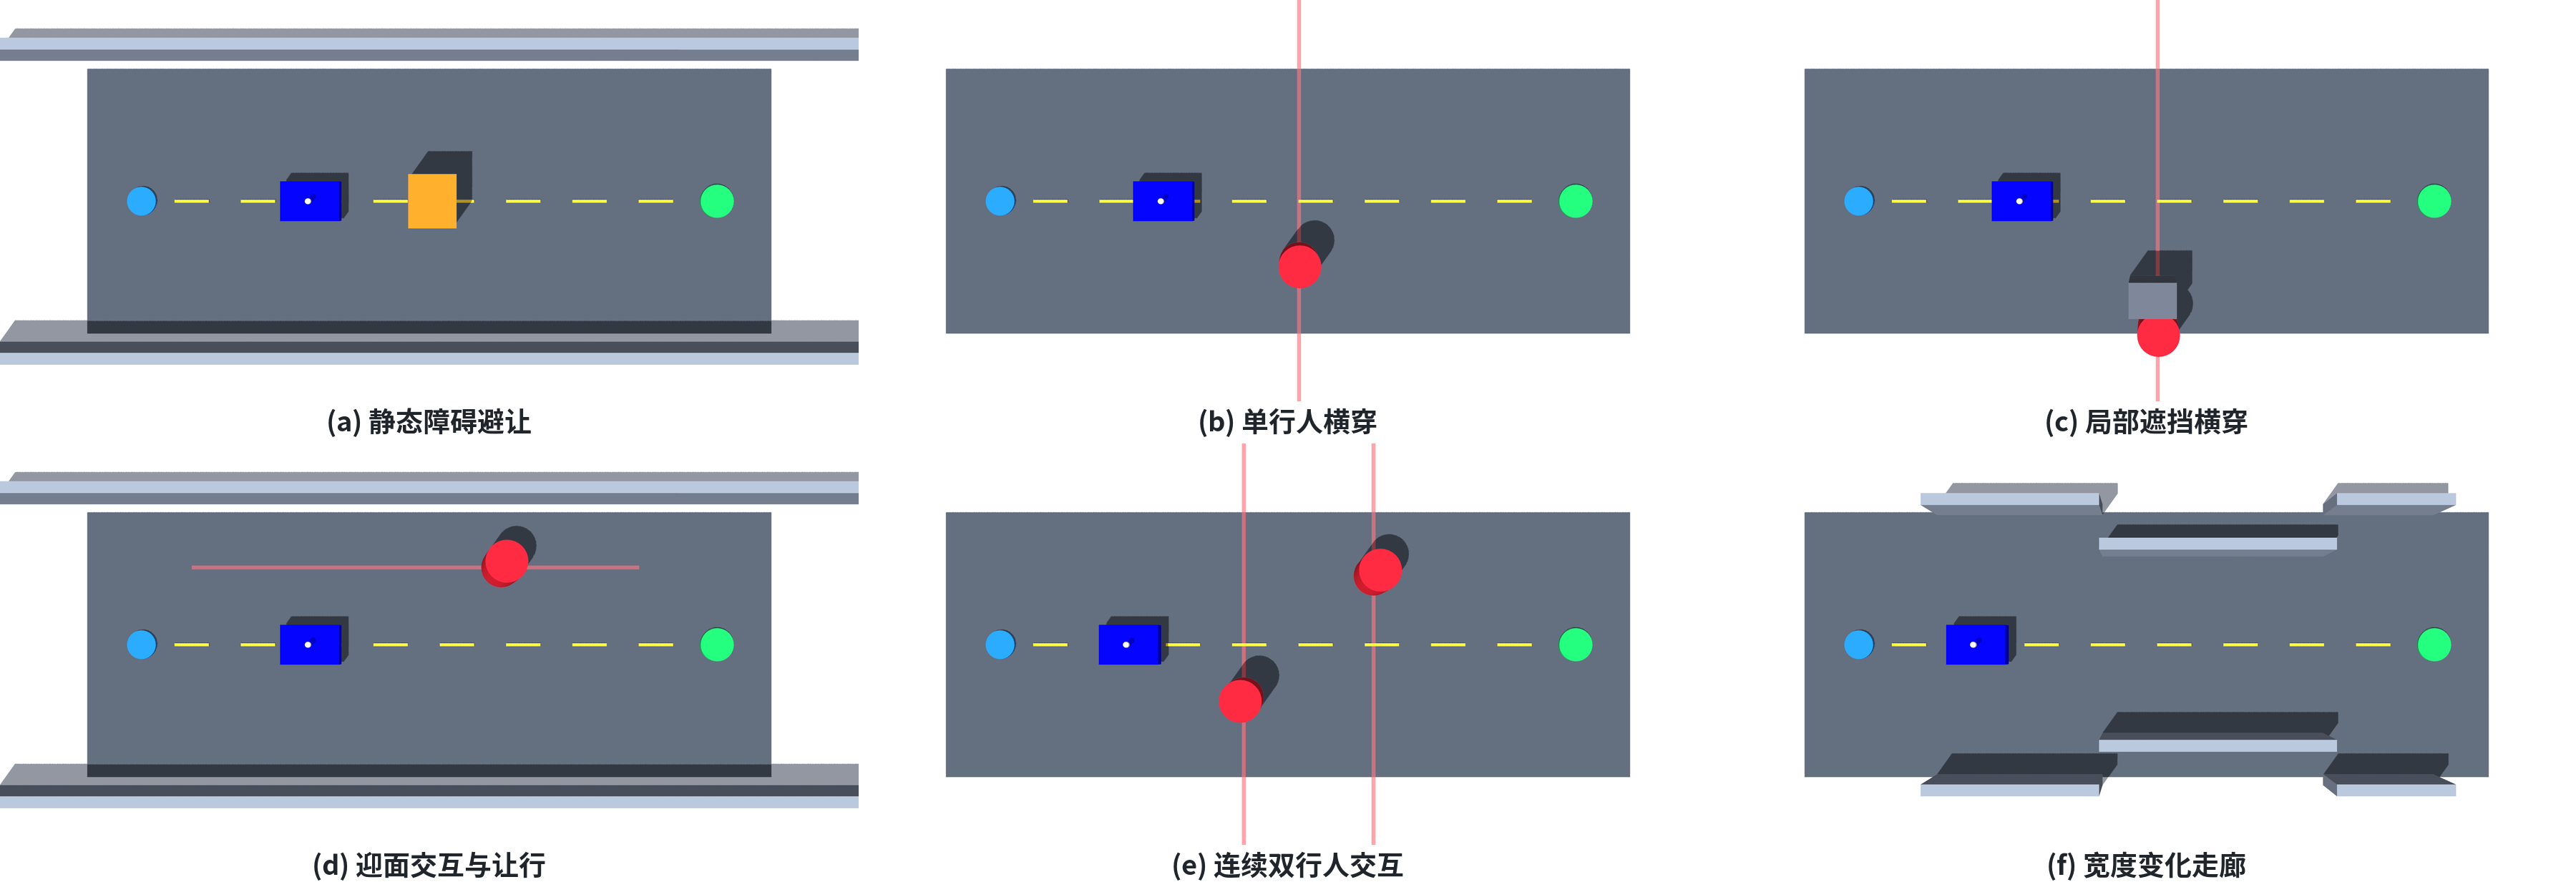
\includegraphics[width=\textwidth]{02_m2_scene_gallery/00_six_scene_overview.png}
  \caption{Gazebo仿真测试场景：（a）静态障碍避让；（b）单行人横穿；（c）局部遮挡横穿；（d）迎面交互与让行；（e）连续双行人交互；（f）宽度变化走廊。}
  \label{fig:gazebo_six_scenes}
\end{figure}

% 2. Arena 五类高细节环境总览
\begin{figure}[htbp]
  \centering
  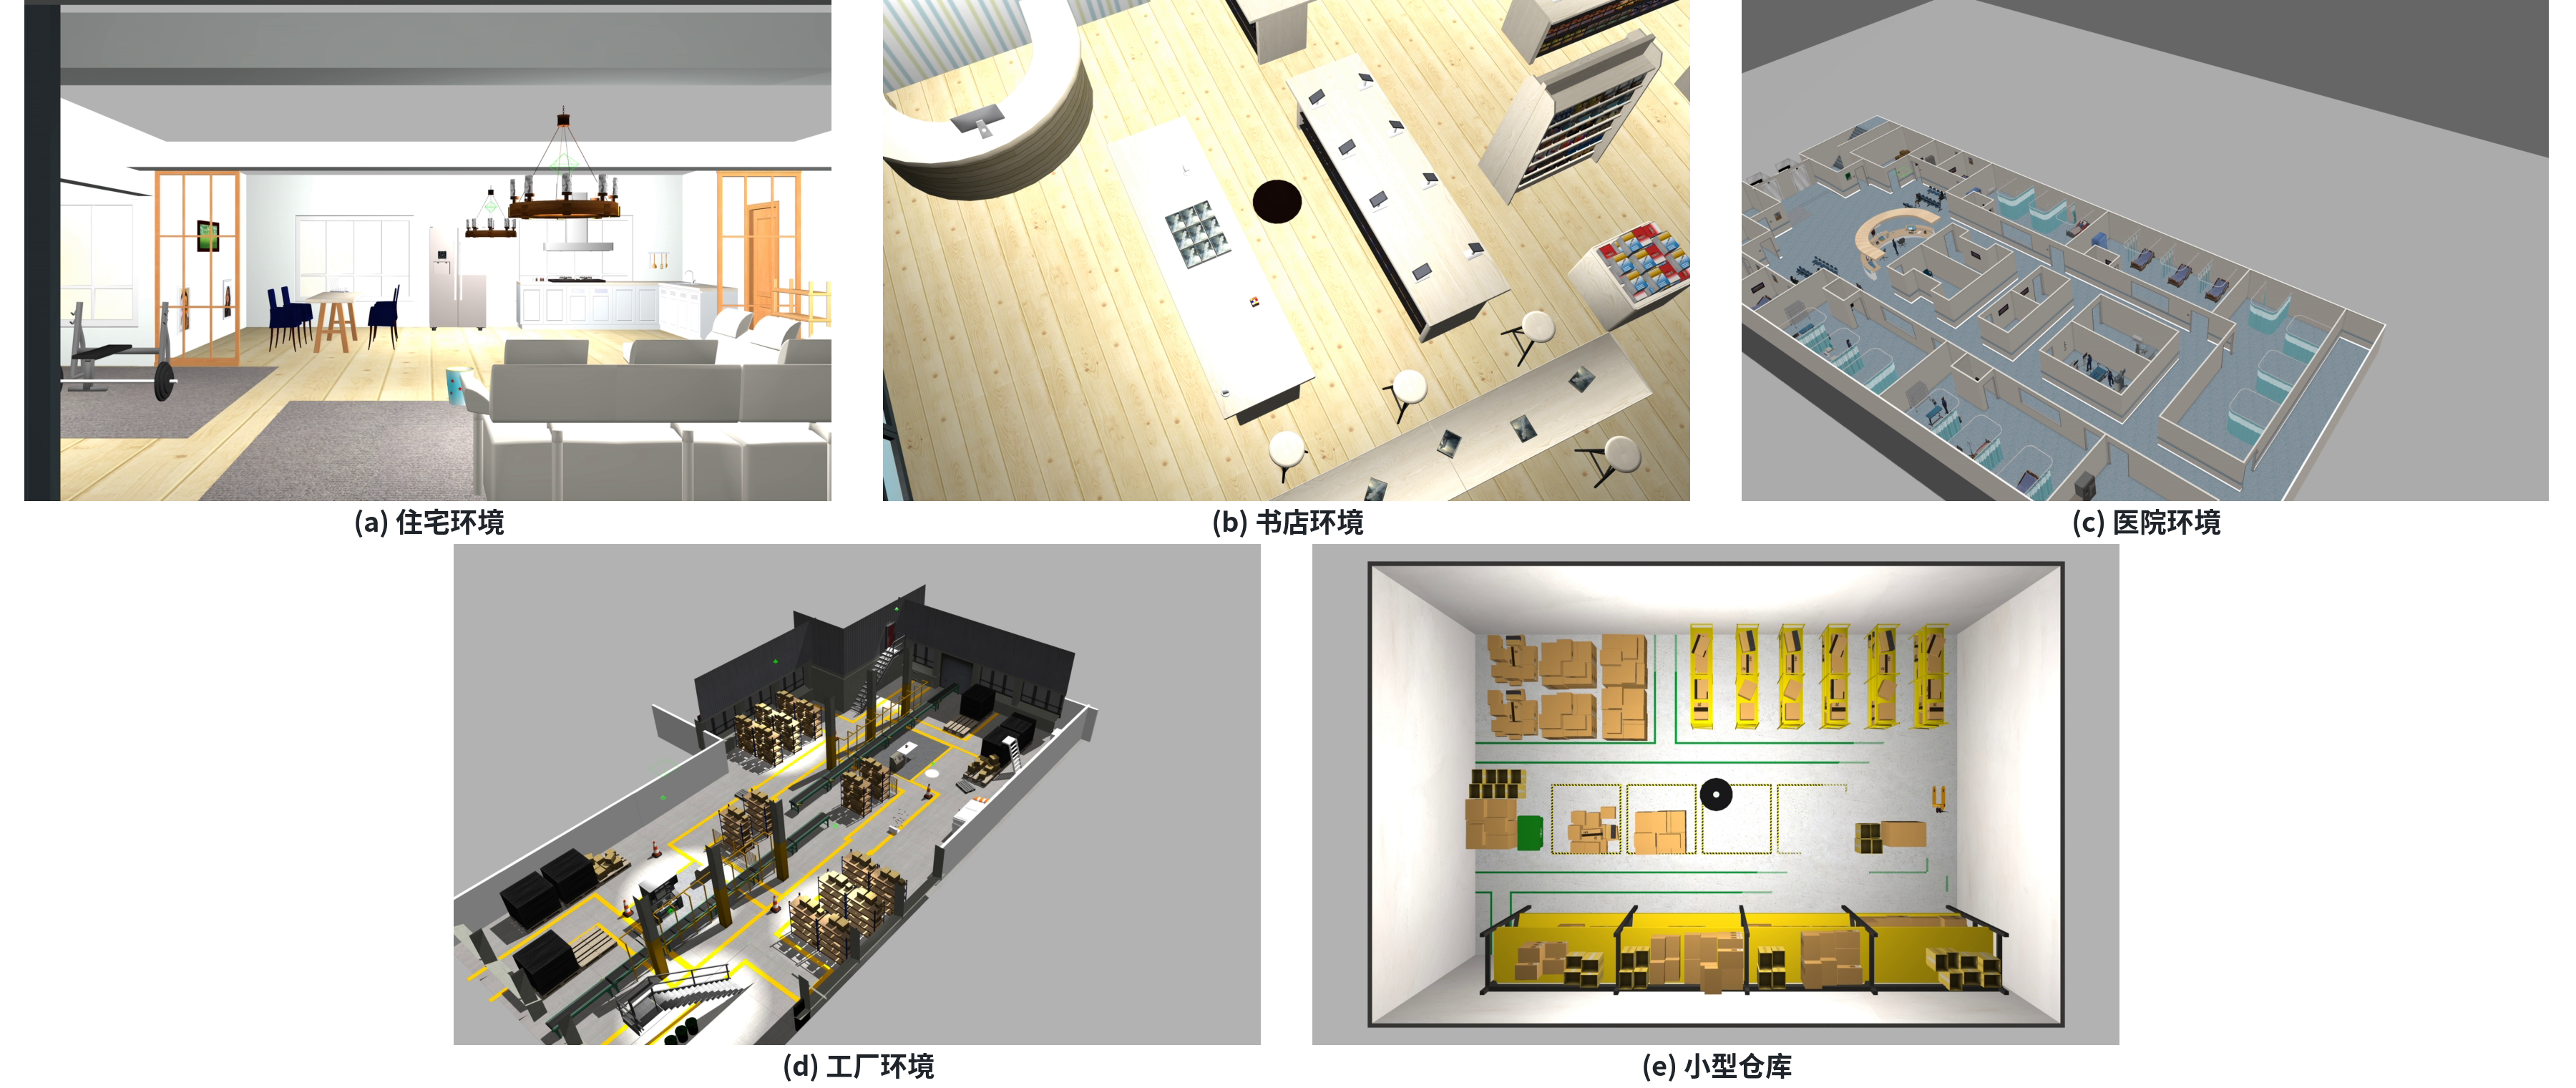
\includegraphics[width=\textwidth]{03_arena_scene_gallery/00_arena_environment_overview.png}
  \caption{Arena-Rosnav-3D集成的多类型三维仿真环境：（a）住宅；（b）书店；（c）医院；（d）工厂；（e）小型仓库。该图为暂停态平台扩展场景示例，非本文冻结正式实验结果。}
  \label{fig:arena_environment_gallery}
\end{figure}

% 3. Gazebo 两轮正式效应图
% 若使用的 LaTeX 工具链支持 SVG，可改用 figures/svg/ 下的同名文件。
\begin{figure}[htbp]
  \centering
  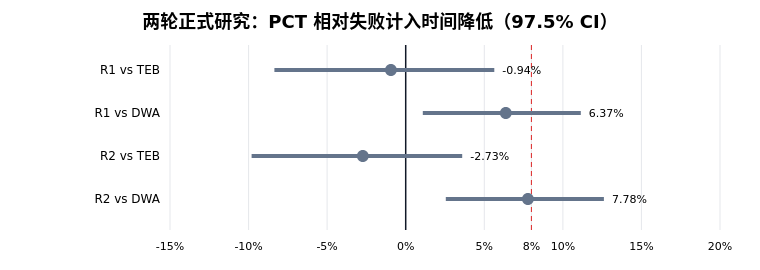
\includegraphics[width=0.90\textwidth]{01_gazebo_formal_comparison/figures/png/formal_effects_97_5_ci.png}
  \caption{两轮正式Gazebo实验中PCT-SCOPE-RL相对传统规划器的失败计入时间效应。点为配对相对降低，误差线为双侧97.5\% block-bootstrap区间，虚线为预注册的8\%点效应门限。两轮均无比较通过全部阳性门限。}
  \label{fig:gazebo_formal_effects}
\end{figure}

% 4. Gazebo R2 方法结果
\begin{figure}[htbp]
  \centering
  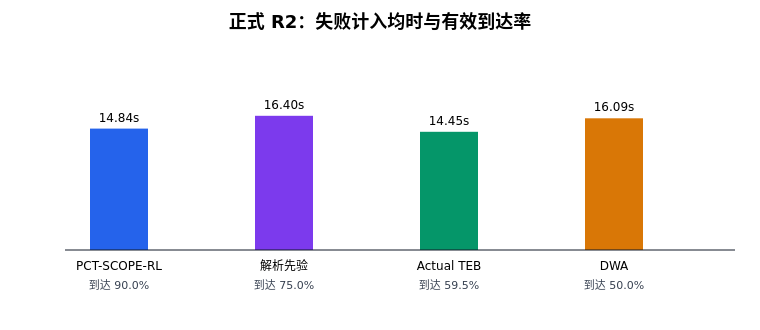
\includegraphics[width=0.90\textwidth]{01_gazebo_formal_comparison/figures/png/formal_r2_method_outcomes.png}
  \caption{R2正式实验中四种方法的失败计入平均时间与有效到达率。失败样本按冻结规则保留并计入。}
  \label{fig:gazebo_r2_outcomes}
\end{figure}

% 5. Arena Hospital 双口径资格结果
\begin{figure}[htbp]
  \centering
  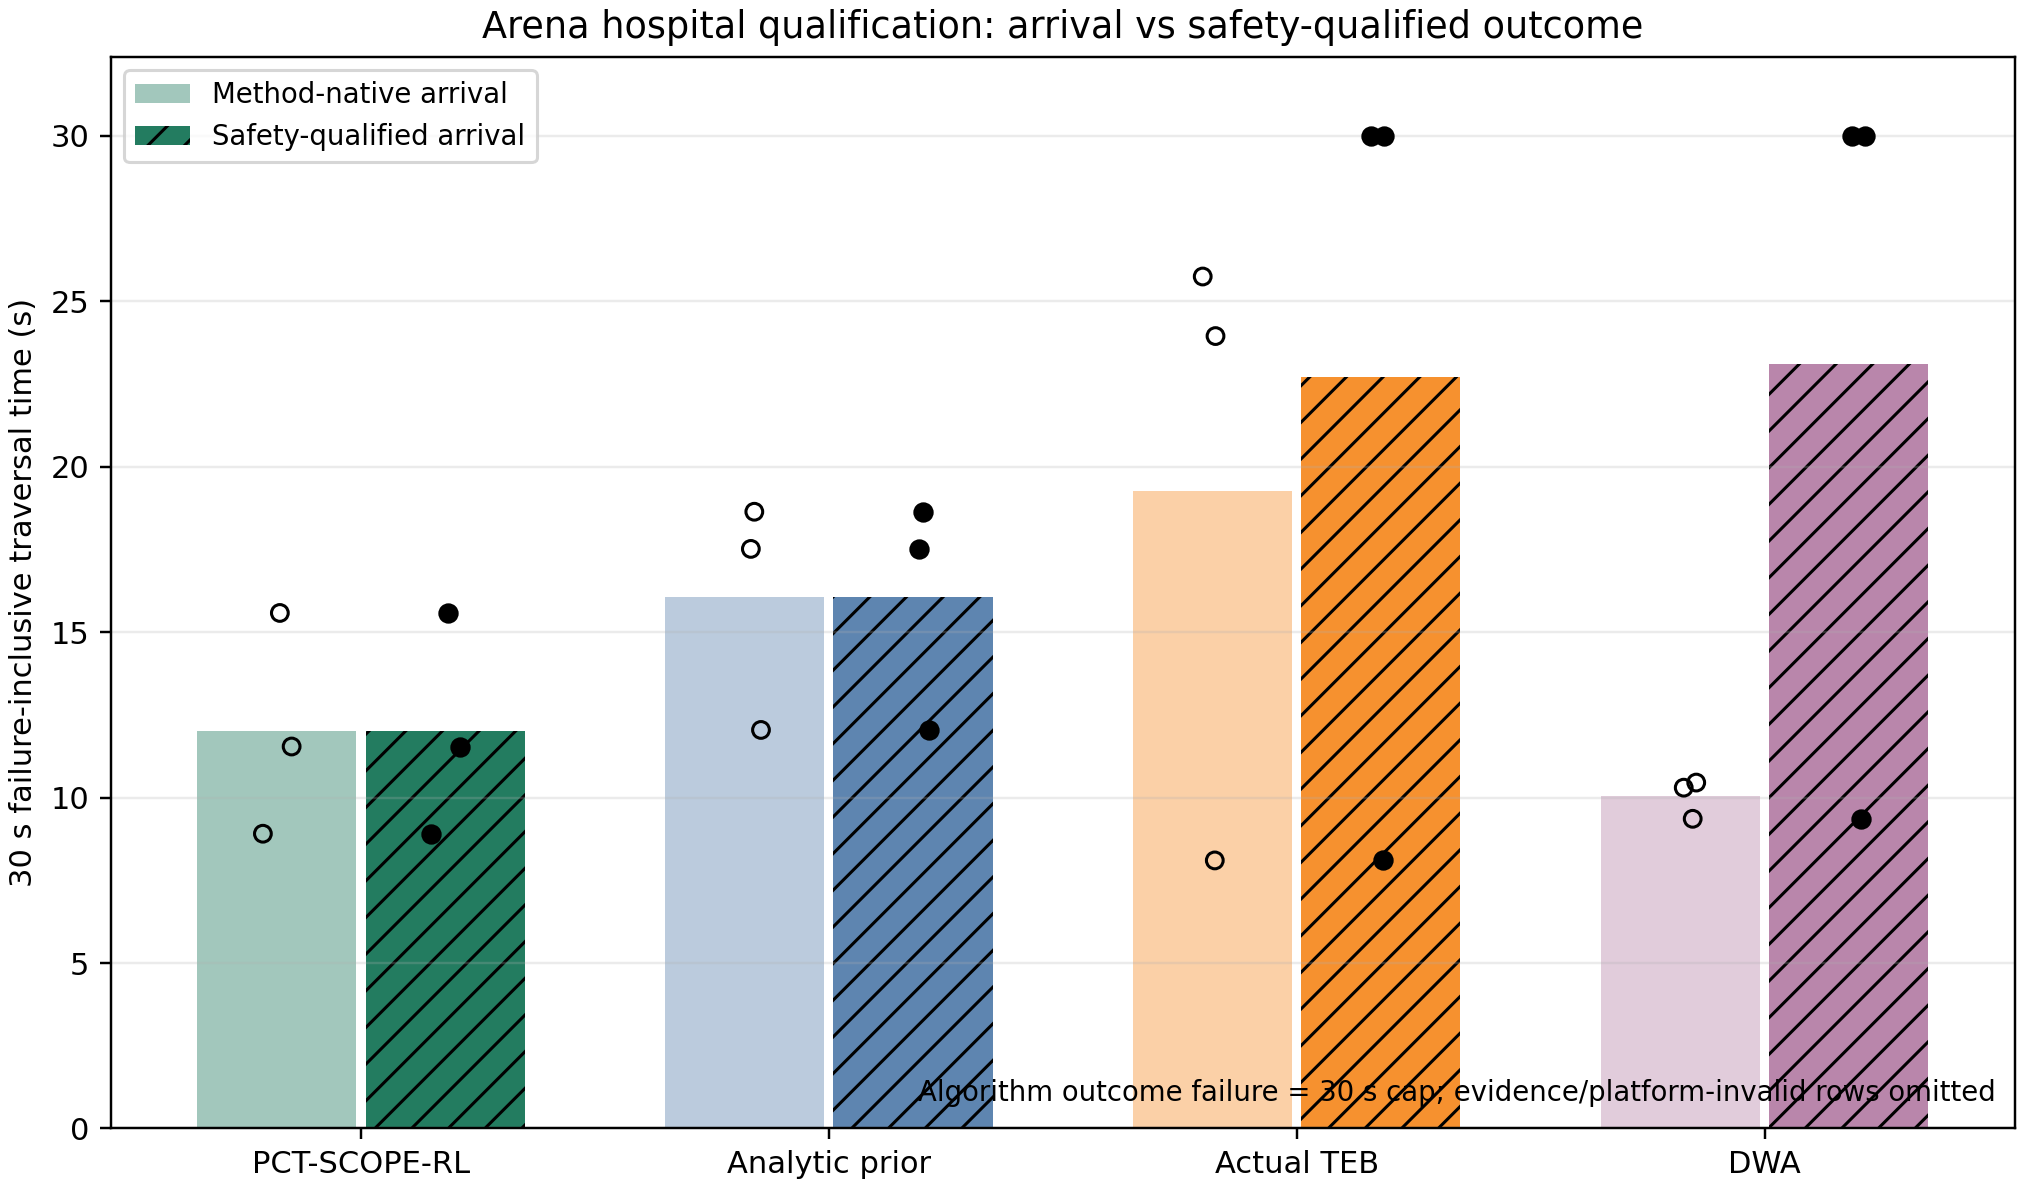
\includegraphics[width=0.88\textwidth]{04_arena_q1_qualification/figures/failure_inclusive_time.png}
  \caption{Arena Hospital资格实验的原始到达与安全规范合格结果。柱高为3个配对块的失败计入平均时间；该结果为描述性资格证据，不包含显著性推断。}
  \label{fig:arena_q1_time}
\end{figure}

% 6. Arena Hospital 执行轨迹
\begin{figure}[htbp]
  \centering
  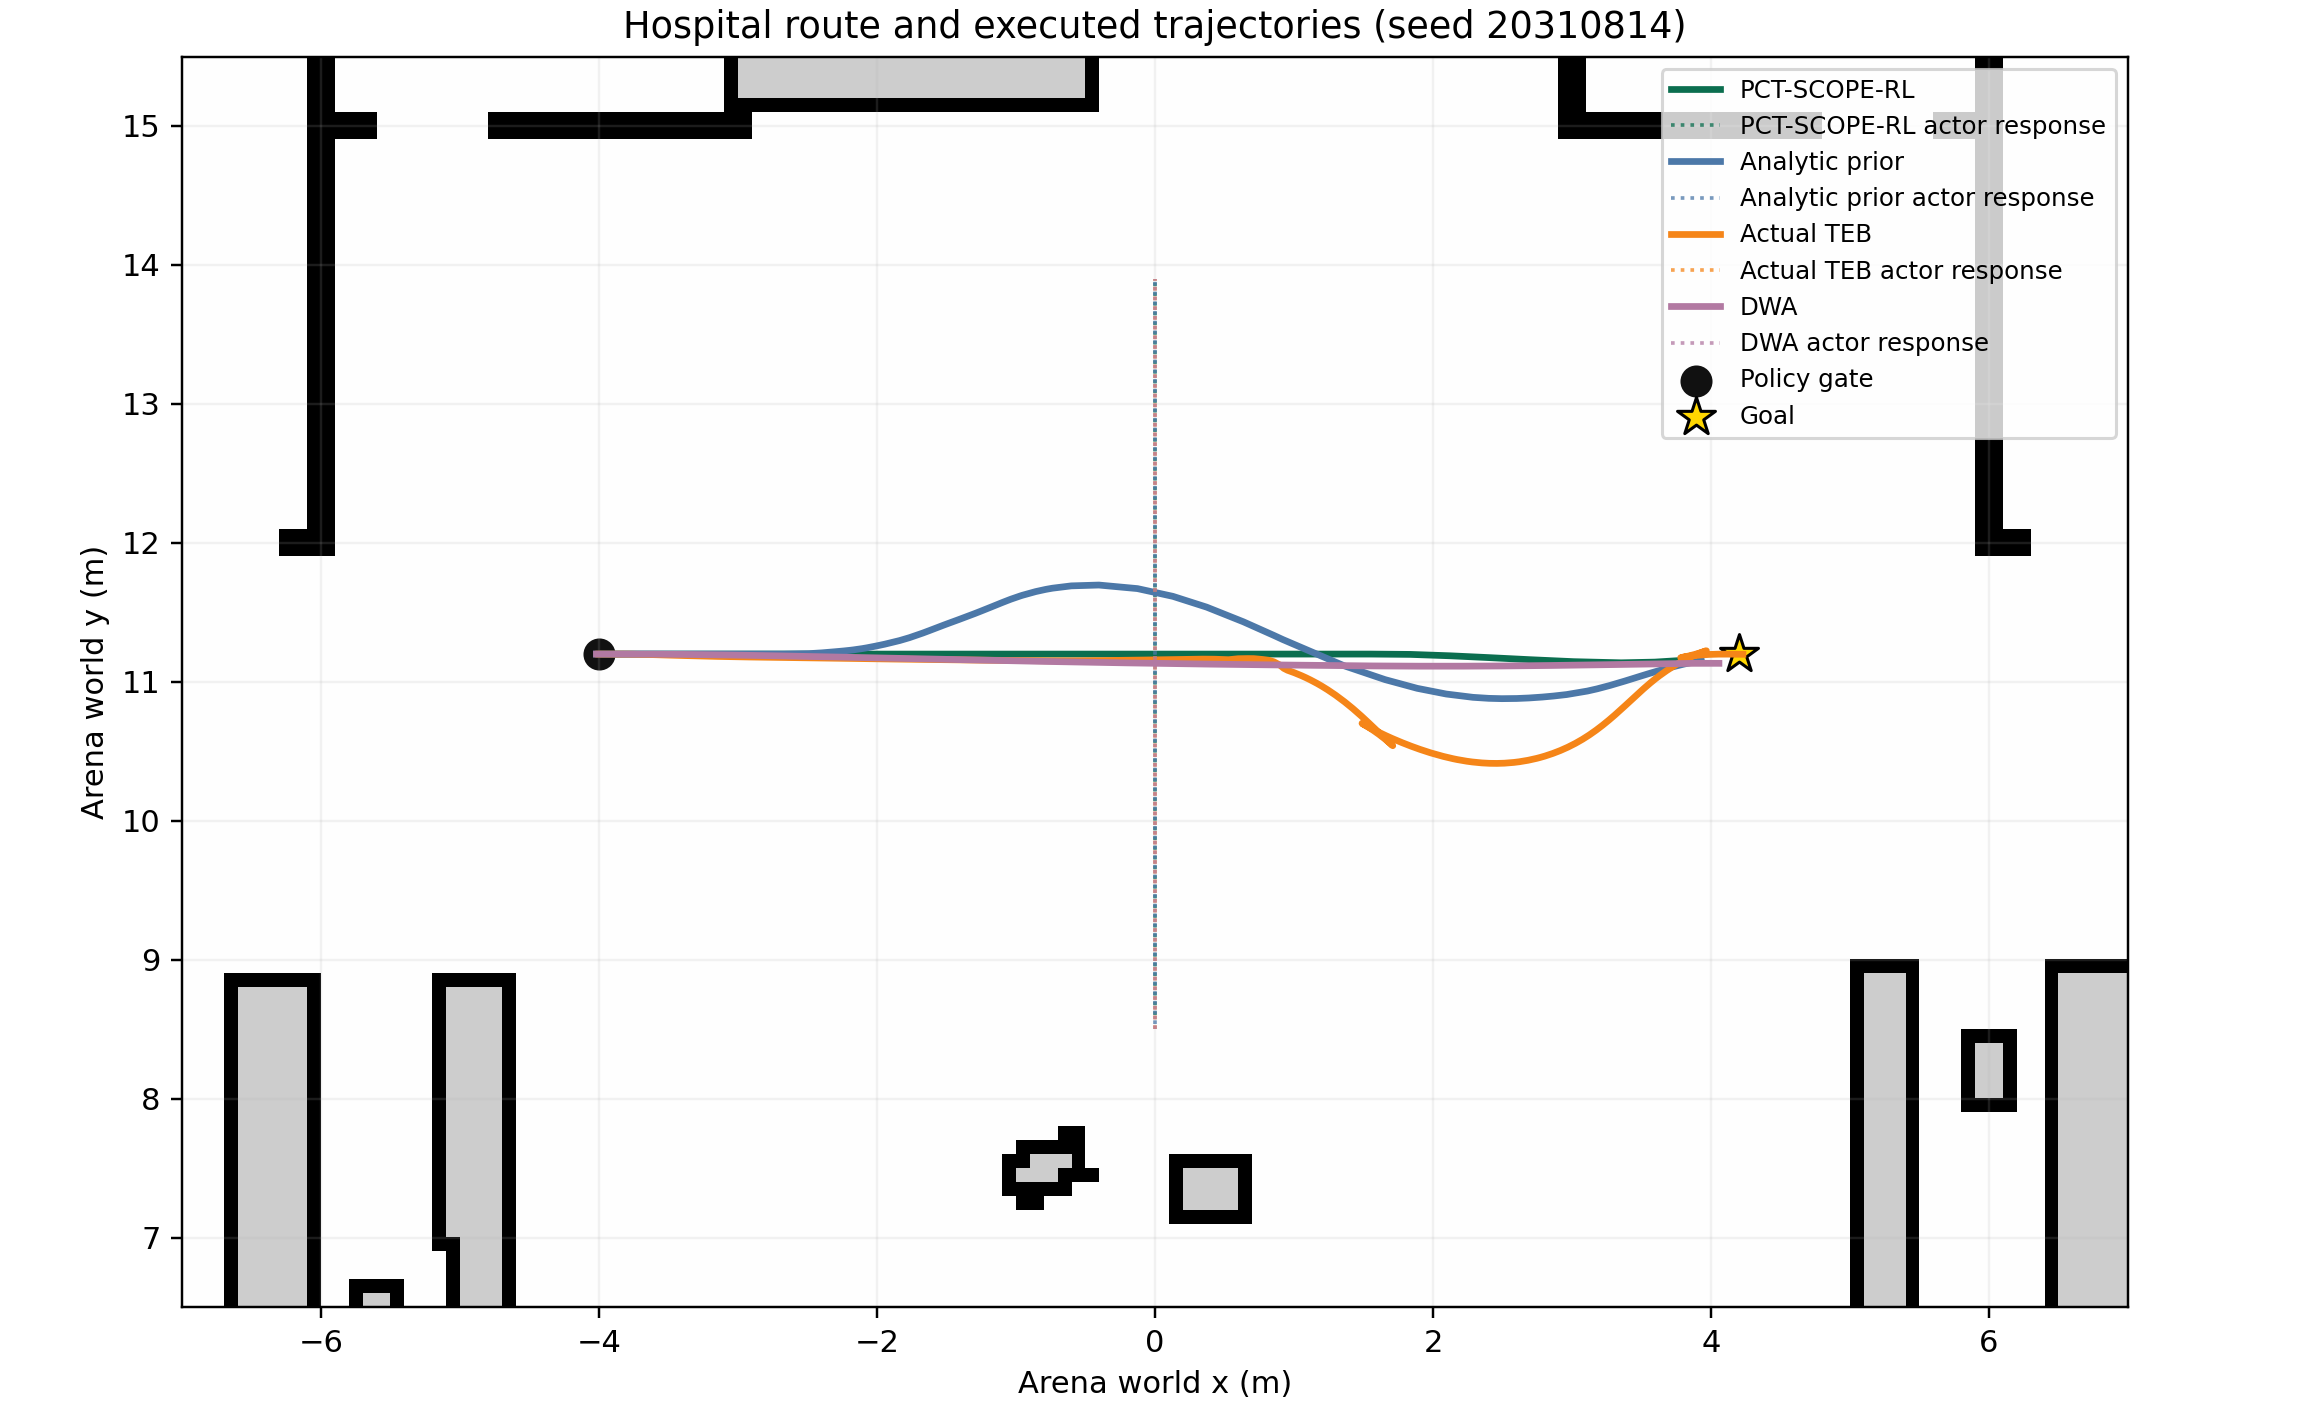
\includegraphics[width=0.90\textwidth]{04_arena_q1_qualification/figures/hospital_route_trajectories.png}
  \caption{Arena Hospital受控横穿任务中的四方法机器人轨迹及方法条件下的闭环反应式代理轨迹。}
  \label{fig:arena_q1_trajectories}
\end{figure}

